% !TeX root=../main.tex

\chapter{مقدمه}
% دستور زیر باعث عدم‌نمایش شماره صفحه در اولین صفحه‌ی این فصل می‌شود.
%\thispagestyle{empty}
\section{آشنایی با این راهنما}
حروف‌چینی پروژه کارشناسی، پایان‌نامه یا رساله یکی از موارد پرکاربرد استفاده از
\lr{\LaTeX}
و زی‌پرشین
\cite{Khalighi87xepersian}
است. یک پروژه، پایان‌نامه یا رساله، احتیاج به تنظیمات زیادی از نظر صفحه‌آرایی دارد که وقت زیادی از دانشجو می‌گیرد. به دلیل قابلیت‌های بسیار لاتک در حروف‌چینی، کلاسی با نام 
\lr{tehran-thesis}
برای حروف‌چینی پروژه‌ها، پایان‌نامه‌ها و رساله‌های دانشگاه تهران، بر مبنای کلاس مشابه
\lr{IUST-Thesis}
تهیه شده است. این کلاس و فایل‌های همراه آن به گونه‌ای طراحی شده است که مطابق با دستورالعمل نگارش و تدوین پایان‌نامه کارشناسی ارشد و دکتری پردیس دانشکده‌های فنی دانشگاه تهران
\cite{UTThesisGuide}
باشد.

دستورالعمل نگارش و تدوین پایان‌نامه دانشگاه تهران به دو مقوله می‌پردازد، اول قالب و چگونگی صفحه‌آرایی پایان‌نامه، مانند اندازه و نوع قلم بخشهای مختلف، چینش فصلها، قالب مراجع و مواردی از این قبیل و دوم محتوای هر فصل پایان‌نامه. 
درصورت استفاده از این کلاس، نیازی نیست که دانشجو نگران مقوله اول باشد و پس از تایپ مطالب خود می‌تواند آنها را با لاتک و ابزار آن اجرا کند تا پایان‌نامه خود را با قالب دانشگاه داشته باشد. همچنین با خواندن این راهنما از ملزومات محتوایی هر فصل پایان‌نامه نیز مطلع خواهد شد.

در ادامهٔ  مقدمهٔ این راهنما، ابتدا چگونگی استفاده از کلاس پایان‌نامه و فایل‌های همراه آن را به صورت فنی شرح می‌دهیم و سپس مطالبی را در مورد ویژگی‌های محتوایی فصل ۱ پایان‌نامه (یعنی مقدمه) خواهیم آورد.
بقیهٔ فصل‌های این راهنما، تنها خصوصیات محتوایی فصول مختلف پایان‌نامه را شرح خواهند داد. نهایتاً جهت یادآوری، در پیوست‌ها مطالبی دربارهٔ آشنایی با دستورات لاتک، مدیریت مراجع در لاتک و چگونگی رسم جداول، نمودارها و الگوریتم‌ها آورده خواهند شد.

\section{چگونگی استفاده از کلاس پایان‌نامه}
کلیه فایل‌های لازم برای حروف‌چینی با کلاس فوق، داخل پوشه‌ای به نام
\lr{tehran-thesis}
قرار داده شده است. توجه داشته باشید که برای استفاده از این کلاس باید فونت‌های
\lr{IRLotusICEE}
و
\lr{IRTitr}
را داشته باشید (که همراه با این کلاس هست و نیاز به نصب نیست).
قلم‌های
\lr{IRLotusICEE}
مستخرج از قلم‌های استاندارد
\lr{IRLotus}
شورای عالی اطلاع‌رسانی%
\footnote{
قلم‌های استاندارد
\lr{IRFonts}
از شورای عالی اطلاع‌رسانی، منطبق بر آخرین نسخه استاندارد یونیکد، استاندارد ملی ۶۲۱۹ و استاندارد
\lr{Adobe Glyph Naming}
هستند.
}
هستند که توسط دکتر بابایی‌زاده اصلاحاتی روی آنها صورت پذیرفته است: تبدیل صفر توپر به صفر توخالی (جهت تمایز بیشتر با نقطه) و اضافه شدن
\textit{\textbf{حالت توپر و ایرانیک توأم}}،
که این موارد در قلم‌های شورای عالی اطلاع‌رسانی وجود ندارد.

\subsection{این همه فایل؟!}
\label{muchFiles}
از آنجایی که یک پایان‌نامه یا رساله، یک نوشته بلند محسوب می‌شود، لذا اگر همه تنظیمات و مطالب پایان‌نامه را داخل یک فایل قرار بدهیم، باعث شلوغی و سردرگمی می‌شود. به همین خاطر، قسمت‌های مختلف پایان‌نامه یا رساله  داخل فایل‌های جداگانه قرار گرفته است. مثلاً تنظیمات پایه‌ای کلاس داخل فایل
\lr{tehran-thesis.cls}، 
قسمت مشخصات فارسی پایان‌نامه داخل 
\lr{faTitle.tex}،
مطالب فصل اول داخل 
\lr{chapter1.tex}
و تنظیمات قابل تغییر توسط کاربر داخل 
\lr{commands.tex}،
قرار داده شده است.
\textbf{
	فایل اصلی این مجموعه، فایل
	\lr{main.tex}
	می‌باشد.
}
% یعنی بعد از تغییر فایل‌های دیگر، برای دیدن نتیجه تغییرات، باید این فایل را اجرا کرد. بقیه فایل‌ها به این فایل، کمک می‌کنند تا بتوانیم خروجی کار را ببینیم.
اگر به فایل 
\lr{main.tex}
دقت کنید، متوجه می‌شوید که قسمت‌های مختلف پایان‌نامه، توسط دستورهایی مانند 
\lr{input}
و
\lr{include}
به فایل اصلی، یعنی 
\lr{main.tex}
معرفی شده‌اند.
با توجه به ساختار محتوایی دستورالعمل، در فایل
\lr{main.tex}
فرض شده که پایان‌نامه یا رساله شما، از ۵ فصل و تعدادی پیوست تشکیل شده است. با اینحال، شما می‌توانید به راحتی فصل‌ها و پیوست‌ها را با صلاحدید اساتید راهنما، کم و زیاد کنید. این کار، بسیار ساده است. فرض کنید بخواهید یک فصل دیگر هم به پایان‌نامه اضافه کنید. برای این کار، کافی است یک فایل با نام دلخواه مثلاً 
\lr{chapter6}
و با پسوند 
\lr{.tex}
بسازید و آن را داخل پوشه 
\lr{tehran-thesis}
قرار دهید و سپس این فایل را با دستور 
\verb!\include{chapter6}!
داخل فایل
\lr{main.tex}
 فراخوانی کنید.

\subsection{از کجا شروع کنم؟}
قبل از هر چیز، باید یک توزیع تِک مناسب مانند تک‌لایو
\lr{(TeXLive)}
را روی سیستم خود نصب کنید. تک‌لایو  را می‌توانید از 
 \href{http://www.tug.org/texlive}{سایت رسمی آن}%
\LTRfootnote{\lr{\url{http://www.tug.org/texlive}}}
 دانلود کنید یا مستقیماً از مخازن توزیع لینوکس خود بگیرید (مثلاً در اوبونتو با دستور
\LRE{\verb!sudo apt install texlive-full!}).
برای نصب تک‌لایو و اجرای اسناد زی‌پرشین می‌توانید از
\href{http://parsilatex.com/site/shop/}{دی‌وی‌دی مجموعه پارسی‌لاتک}%
\LTRfootnote{\lr{\url{http://parsilatex.com/site/shop/}}}
و فایل راهنمای موجود در آن هم کمک بگیرید.

برای تایپ و پردازش اسناد لاتک باید از یک ویرایشگر مناسب استفاده کنید. ویرایشگرهای
\lr{TeXWroks},
\lr{TeXstudio},
\lr{Texmaker}
و
\lr{BiDiTeXmaker}
بدین منظور تولید شده‌اند. می‌توان ویرایش‌گر 
 \href{https://bitbucket.org/srazi/biditexmaker3}{\lr{BiDiTeXmaker}}%
 \LTRfootnote{\lr{\url{https://bitbucket.org/srazi/biditexmaker3}}}
را که بویژه برای کار با زی‌پرشین و مطالب دوجهته بهبود یافته است، بهینه‌ترین ویرایشگر لاتک برای کار با اسناد فارسی عنوان کرد.
 
حال اگر نوشتن \پ اولین تجربه شما از کار با لاتک است، توصیه می‌شود که یک‌بار به صورت اجمالی، کتاب «%
\href{http://www.tug.ctan.org/tex-archive/info/lshort/persian/lshort.pdf}{مقدمه‌ای نه چندان کوتاه بر
\lr{\LaTeXe}}%
\LTRfootnote{\lr{\url{http://www.tug.ctan.org/tex-archive/info/lshort/persian/lshort.pdf}\hfill}}»
ترجمه دکتر مهدی امیدعلی را مطالعه کنید. این کتاب، کتاب بسیار کاملی است که خیلی از نیازهای شما در ارتباط با حروف‌چینی را برطرف می‌کند.
اگر تک لایو کامل را داشته باشید، این کتاب را هم دارید. کافیست در خط فرمان دستور زیر را بزنید:
\begin{latin}
	\texttt{texdoc lshort-persian}
\end{latin}
اگر عجله دارید، برخی دستورات پایه‌ای مورد نیاز در پیوست \ref{app:latexIntro} بیان شده‌اند.
 
بعد از موارد گفته شده، فایل 
\lr{main.tex}
و
\lr{faTitle.tex}
را باز کنید و مشخصات پایان‌نامه خود مثل نام، نام خانوادگی، عنوان پایان‌نامه و ... را جایگزین مشخصات موجود در فایل
\lr{faTitle.tex}
 کنید. نیازی نیست نگران چینش این مشخصات در فایل پی‌دی‌اف خروجی باشید، زیرا کلاس 
\lr{tehran-thesis}
همه این کارها را بطور خودکار برای شما انجام می‌دهد. در ضمن، موقع تغییر دادن دستورهای داخل فایل
\lr{faTitle.tex}
 کاملاً دقت کنید؛ این دستورها، خیلی حساس هستند و ممکن است با یک تغییر کوچک، موقع اجرا، خطا بگیرید. برای دیدن خروجی کار، فایل 
\lr{faTitle.tex}
 را 
\lr{Save}
(نه 
\lr{Save As})
کنید و بعد به فایل 
\lr{main.tex}
برگشته و آن را اجرا کنید%
\footnote{
	البته فایلهای این مجموعه به گونه‌ای هستند که در
	\lr{TeXWorks} یا
	\lr{TeXstudio}
	بدون بازگشت به فایل اصلی، می‌توانید سند خود را اجرا کنید.
}.
 حال اگر می‌خواهید مشخصات انگلیسی \پ را هم عوض کنید، فایل 
\lr{enTitle.tex}
را باز کنید و مشخصات داخلش را تغییر دهید.
%\RTLfootnote{
%برای نوشتن پروژه کارشناسی، نیازی به وارد کردن مشخصات انگلیسی پروژه نیست. بنابراین، این مشخصات بطور خودکار، نادیده گرفته می‌شود.
%}
در اینجا هم برای دیدن خروجی باید این فایل را ذخیره کرده، بعد به فایل 
\lr{main.tex}
برگشته و آن را اجرا کرد.

برای راحتی بیشتر، کلاس 
\lr{tehran-thesis.cls}
طوری طراحی شده است که کافی است فقط  یک‌بار مشخصات \پ را (در فایل‌های
\lr{faTitle.tex}
و
\lr{enTitle.tex})
وارد کنید و هر جای دیگر که این مشخصات لازم باشند، به طور خودکار درج می‌شوند. با این حال، اگر مایل بودید، می‌توانید تنظیمات موجود را تغییر دهید؛ گرچه، در صورتیکه کاربر مبتدی هستید و یا با ساختار فایل‌های  
\lr{cls}
 آشنایی ندارید، بهتر است به فایل 
\lr{tehran-thesis.cls}
دست نزنید.

نکته دیگری که باید به آن توجه کنید این است که در قالب آماده شده، سه گزینه به نام‌های
\lr{bsc}،
\lr{msc}
و
\lr{phd}
برای نوشتن پروژه، پایان‌نامه و رساله، در نظر گرفته شده است. بنابراین اگر قصد تایپ پروژهٔ کارشناسی، پایان‌نامهٔ کارشناسی ارشد یا رسالهٔ دکتری را دارید، به ترتیب باید از گزینه‌های
\lr{bsc}،
\lr{msc}
و
\lr{phd}
در فایل 
\lr{main.tex}
استفاده کنید. با انتخاب هر کدام از این گزینه‌ها، تنظیمات مربوط به آنها به طور خودکار، اعمال می‌شود.


\subsection[مطالب پایان‌نامه را چطور بنویسم؟]
{مطالب \پ را چطور بنویسم؟}
\subsubsection{نوشتن فصل‌ها}
همان‌طور که در بخش \ref{muchFiles} گفته شد برای جلوگیری از شلوغی، قسمت‌های مختلف \پ از جمله فصل‌ها، در فایل‌های جداگانه‌ای قرار داده شده‌اند. 
مثلاً اگر می‌خواهید مطالب فصل ۱ را تایپ کنید، باید فایل‌های 
\lr{main.tex}
و
\lr{chapter1.tex}
را باز کرده و مطالب خود را جایگزین محتویات داخل 
\lr{chapter1.tex}
نمایید. دقت شود که در ابتدای برخی فایلها دستوراتی نوشته شده است و از شما خواسته شده که آن دستورات را حذف نکنید.

%توجه کنید که همان‌طور که قبلاً هم گفته شد، تنها فایل قابل اجرا، 
%\lr{main.tex}
%است. لذا برای دیدن حاصل (خروجی) فایل خود، باید  
%\lr{chapter1.tex}
%را ذخیره کرده و سپس فایل 
%\lr{main.tex}
%را اجرا کنید.

نکته بسیار مهمی که در اینجا باید گفته شود این است که سیستم \lr{\TeX}، محتویات یک فایل تِک را به ترتیب پردازش می‌کند.  بنابراین، اگر مثلاً  دو فصل اول خود را نوشته و خروجی آنها را دیده‌اید و مشغول تایپ مطالب فصل ۳ هستید، بهتر است
که دو دستور 
\verb!\chapter{مقدمه}
\section{مقدمه ای بر ساختار \lr{ORAN}}
\lr{Open RAN}(\lr{ORAN})
تبسیط و ترکیبی از دو ساختار \lr{C-RAN} و \lr{xRAN} می باشد که انتظار می رود که در فناوری نسل پنجم مخابرات مورد استفاده قرار گرفته و منجر به بهبود عملکرد شبکه های دسترسی رادیویی \lr{RAN} گردد. 
ایده اصلی \lr{C-RAN} جداسازی بخش  
!
و
\verb!% !TeX root=../main.tex
\chapter{مروری بر مطالعات انجام شده}
%\thispagestyle{empty} 
\section{مقدمه}
هدف از این فصل که با عنوان‌های  «مروری بر ادبیات موضوع%
\LTRfootnote{Literature Review}»،
«مروری بر منابع» و یا «مروری بر پیشینه تحقیق%
\LTRfootnote{Background Research}»
معرفی می‌شود، بررسی و طبقه‌بندی یافته‌های تحقیقات دیگر محققان در سطح دنیا و تعیین و شناسایی خلأهای تحقیقاتی است. آنچه را که تحقیق شما به دانش موجود اضافه می‌کند، مشخص کنید. طرح پیشینه تحقیق%
\LTRfootnote{Background Information}
یک مرور محققانه است و تا آنجا باید پیش برود که پیش‌زمینهٔ تاریخی مناسبی از تحقیق را بیان کند و جایگاه تحقیق فعلی را در میان آثار پیشین نشان دهد. برای این منظور منابع مرتبط با تحقیق را بررسی کنید، البته نه آنچنان گسترده که کل پیشینه تاریخی بحث را در برگیرد. برای نوشتن این بخش:
\begin{itemize}
	\item
	دانستنی‌های موجود و پیش‌زمینهٔ تاریخی و وضعیت کنونی موضوع را چنان بیان کنید که خواننده بدون مراجعه به منابع پیشین، نتایج حاصل از مطالعات قبلی را درک و ارزیابی کند.
	\item
	نشان دهید که بر موضوع احاطه دارید. پرسش تحقیق را همراه بحث و جدل‌ها و مسائل مطرح شده بیان کنید و مهم‌ترین تحقیق‌های انجام شده در این زمینه را معرفی نمائید.
	\item
	ابتدا مطالب عمومی‌تر و سپس پژوهش‌های مشابه با کار خود را معرفی کرده و نشان دهید که تحقیق شما از چه جنبه‌ای با کار دیگران تشابه یا تفاوت دارد.
	\item
	اگر کارهای قبلی را خلاصه کرده‌اید، از پرداختن به جزئیات غیرضروری بپرهیزید. در عوض، بر یافته‌ها و مسائل روش‌شناختی مرتبط و نتایج اصلی تأکید کنید و اگر بررسی‌ها و منابع مروری عمومی دربارهٔ موضوع موجود است، خواننده را به آنها ارجاع دهید.
\end{itemize}

\section{تعاریف، اصول و مبانی نظری}
این قسمت ارائهٔ خلاصه‌ای از دانش کلاسیک موضوع است. این بخش الزامی نیست و بستگی به نظر استاد راهنما دارد.

\section{مروری بر ادبیات موضوع}
در این قسمت باید به کارهای مشابه دیگران در گذشته اشاره کرد و وزن بیشتر این قسمت بهتر است به مقالات ژورنالی سال‌های اخیر (۲ تا ۳ سال) تخصیص داده شود. به نتایج کارهای دیگران با ذکر دقیق مراجع باید اشاره شده و جایگاه و تفاوت تحقیق شما نیز با کارهای دیگران مشخص شود. استفاده از مقالات ژورنال‌های معتبر در دو یا سه سال اخیر، می‌تواند به اعتبار کار شما بیافزاید.

\section{نتیجه‌گیری}
‌در نتیجه‌گیری آخر این فصل، با توجه به بررسی انجام شده بر روی مراجع تحقیق، بخش‌های قابل گسترش و تحقیق در آن حیطه و چشم‌اندازهای تحقیق مورد بررسی قرار می‌گیرند.	در برخی از تحقیقات، نتیجه نهایی فصل روش تحقیق، ارائهٔ یک چارچوب کار تحقیقی 
\lr{(research framework)}
است.!
را در فایل 
\lr{main.tex}،
غیرفعال%
\footnote{
برای غیرفعال کردن یک دستور، کافی است در ابتدای آن، علامت درصد انگلیسی (\%) بگذارید.
}
 کنید. در غیر این صورت، ابتدا مطالب دو فصل اول پردازش شده و سپس مطالب فصل ۳ پردازش می‌شود که این کار باعث طولانی شدن زمان پردازش می‌گردد. هر زمان که خروجی کل \پ را خواستید، تمام فصل‌ها را دوباره در
\lr{main.tex}
فعال نمائید.
بدیهتاً لازم نیست فصل‌های \پ را به ترتیب تایپ کنید. مثلاً می‌توانید ابتدا مطالب فصل ۳ را تایپ نموده و سپس مطالب فصل ۱ را تایپ کنید. 
\subsubsection{مراجع}
برای وارد کردن مراجع \پ کافی است فایل 
\lr{MyReferences.bib}
را باز کرده و مراجع خود را به شکل اقلام نمونهٔ داخل آن، وارد کنید.  سپس از \lr{bibtex} برای تولید مراجع با قالب مناسب استفاده نمائید. برای توضیحات بیشتر بخش \ref{Sec:Ref} از پیوست \ref{app:latexIntro} و نیز پیوست \ref{app:refMan} را ببینید.

\subsubsection{واژه‌نامه فارسی به انگلیسی و برعکس}
برای وارد کردن معادل فارسی اصطلاحات لاتین در متن و تهیه فهرست واژه‌نامه از آنها، از بستهٔ
\lr{glossaries}
و نرم‌افزار
\lr{xindy}
استفاده می‌شود. بدین منظور کافی است اصطلاحات لاتین و ترجمهٔ آنها را در فایل
\lr{words.tex}
وارد کرده و هر جای متن که خواستید با دستورات
\verb|gls{label}|
یا \verb|glspl{label}|
معادل فارسی مفرد یا جمع یک اصطلاح را بیاورید.

مثلا در اینجا، واژهٔ
«\gls{Action}»
برای بار اول و دوباره
«\gls{Action}»
برای بار دوم در متن ظاهر شده است.
جهت توضیحات بیشتر به پیوست
\ref{app:refMan}
مراجعه کنید.
\subsubsection{نمایه}
برای وارد کردن نمایه، باید از 
\lr{xindy}
استفاده کنید. 
%زیرا 
%\lr{MakeIndex}
%با حروف «گ»، «چ»، «پ»، «ژ» و «ک» مشکل دارد و ترتیب الفبایی این حروف را رعایت نمی‌کند. همچنین، فاصله بین هر گروه از کلمات در 
%\lr{MakeIndex}،
%به درستی رعایت نمی‌شود که باعث زشت شدن حروف‌چینی این قسمت می‌شود. 
راهنمای چگونگی کار با 
\lr{xindy} 
را می‌توانید در ویکی پارسی‌لاتک و یا مثالهای موجود در دی‌وی‌دی «مجموعه پارسی‌لاتک»، پیدا کنید.

\subsection{اگر سوالی داشتم، از کی بپرسم؟}
برای پرسیدن سوال‌های خود موقع حروف‌چینی با زی‌پرشین، می‌توانید به
\href{http://qa.parsilatex.com}{سایت پرسش و پاسخ پارسی‌لاتک}%
\LTRfootnote{http://qa.parsilatex.com}
یا
\href{http://forum.parsilatex.com}{بایگانی تالارگفتگوی قدیمی پارسی‌لاتک}%
\LTRfootnote{http://forum.parsilatex.com}
مراجعه کنید. شما هم می‌توانید روزی به سوال‌های دیگران در اینترنت جواب دهید.
بستهٔ زی‌پرشین و بسیاری از بسته‌های مرتبط با آن مانند
\lr{bidi} و
\lr{Persian-bib}،
مجموعه پارسی‌لاتک، مثالهای مختلف موجود در آن، قالب پایان‌نامه دانشگاههای مختلف و سایت پارسی‌لاتک همه به صورت داوطلبانه توسط افراد گروه پارسی‌لاتک و گروه
\lr{Persian TeX}
و بدون هیچ کمک مالی انجام شده‌اند. کار اصلی نوشتن و توسعه زی‌پرشین توسط آقای وفا خلیقی انجام شده است که این کار بزرگ را به انجام رساندند.
اگر مایل به کمک به گروه پارسی‌لاتک هستید به سایت این گروه مراجعه فرمایید:
\begin{center}
	\url{http://www.parsilatex.com}
\end{center}

\section{محتویات فصل اول یک پایان‌نامه}
فصل اول یک پایان‌نامه باید به مقدمه یا کلیات تحقیق بپردازد.
هدف از فصل مقدمه%
\LTRfootnote{Introduction}،
شرح مختصر مسأله تحقیق، اهمیت و انگیزه محقق از پرداختن به آن موضوع، بهمراه اشاره‌ای کوتاه به روش و مراحل تحقیق است. مقدمه، اولین فصل از ساختار اصلی \پ بوده و زمینه اطلاعاتی لازم را برای خواننده فراهم می‌آورد. در طول مقدمه باید سعی شود موضوع تحقیق با زبانی روشن، ساده و بطور عمیق و هدفمند به خواننده معرفی شود. این فصل باید خواننده را مجذوب و اهمیت موضوع تحقیق را آشکار سازد. در مقدمه باید با ارائهٔ سوابق، شواهد تحقیقی و اطلاعات موجود (با ذکر منبع) با روشی منظم، منطقی و هدف‌دار، خواننده را جهت داد و به سوی راه حل مورد نظر هدایت کرد. مقدمه مناسب‌ترین جا برای ارائهٔ اختصارات و بعضی توضیحات کلی است، توضیحاتی که شاید نتوان در مباحث دیگر آنها را شرح داد.

مقدمه، یکی از ارکان اساسی و اصلی پایان نامه است که مهمترین قسمت‌های آن عبارتند از: 

\subsection{عنوان تحقیق} 
باید شناختی دقیق و روشن از حوزهٔ موضوع تحقیق را عرضه دارد و خالی از هرگونه ابهام و پیچیدگی باشد.

\subsection{مسأله تحقیق}
وظیفه اصلی مقدمه بیان این مطلب به خواننده است که چرا انجام تحقیق را به عهده گرفته‌اید. اگر دلیل شما برای انجام این کار پاسخگویی به سؤال مورد علاقه‌تان است، با مشکل زیادی روبه‌رو نخواهید بود. یکی از بهترین روش‌ها برای نوشتن مقدمهٔ یک پایان‌نامه، طرح پرسش یا پرسش‌هایی مهم و اساسی است که کار تحقیقاتی شما از آغاز تا پایان قصد پاسخ دادن به آن را دارد. گاهی می‌توانید ابتدا اهمیت موضوع را بیان و سپس پرسش خود را در آن موضوع مطرح کنید.

\subsection{تاریخچه‌ای از موضوع تحقیق}
به طور کلی تشریح روندهای تحقیقاتی در محدودهٔ مورد مطالعه، مستلزم ارجاع به کارهای دیگران است. بعضی از نویسندگان برای کارهای دیگران هیچ اعتباری قائل نمی‌شوند و در مقابل، بعضی دیگر از نویسندگان در توصیف کارهای دیگران، بسیار زیاده‌روی می‌کنند. اکثر مواقع، ارجاع به مقالات دو سال قبل از کارتان، بهتر از نوشتن سطرهای مرجع است. در این قسمت باید به طور مختصر به نظرات و تحقیقات مربوط به موضوع و یا مسائل و مشکلات حل نشده در این حوزه و همچنین توجه و علاقه جامعه به این موضوع، اشاره شود.

\subsection{تعریف موضوع تحقیق}
در این قسمت محقق، موضوع مورد علاقه و یا نیاز احساس شدهٔ خود را در حوزه تحقیق بیان می‌دارد و عوامل موجود در موقعیت را تعریف و تعیین می‌کند.

\subsection{هدف یا هدف‌های کلی و آرمانی تحقیق}
این قسمت باید با جملات مثبت و کلی طرح شود و از طولانی شدن مطالب پرهیز شود.

\subsection{روش انجام تحقیق}
در این قسمت، پژوهشگر روش کاری خود را بیان می‌دارد و شیوه‌های گوناگونی را که در گردآوری مطالب خود بکار برده، ذکر می‌کند. همچنین اگر روش آماری خاصی را در تهیه و تدوین اطلاعات به کار برده است، آن شیوه را نیز اینجا بیان می‌کند.

\subsection{نوآوری، اهمیت و ارزش تحقیق}
در این قسمت، در مورد نوآوری علمی و عملی تحقیق که محقق به آن دست خواهد یافت، بحث می‌شود. ممکن است لازم باشد تا برخی نمودارهای خلاصه در این بخش استفاده شوند. به عنوان مثال، نموداری از مقاله
\cite{kim2016integrated}
در شکل
\ref{fig:sampleDiagram}
آمده است.
\begin{figure}[ht]
	\centerline{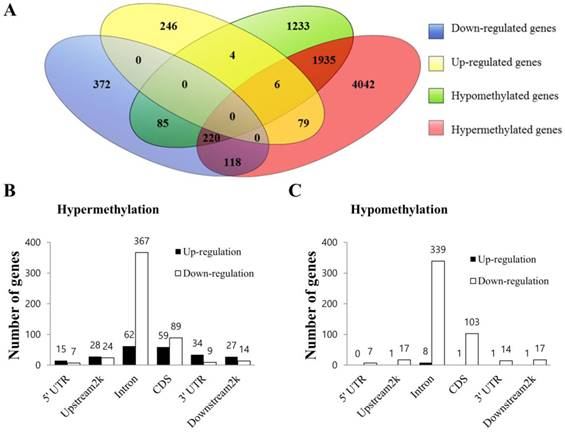
\includegraphics[width=0.8\textwidth]{journal-of-cancer_sample-result}}
	\caption{یک نمونه نمودار خلاصه برای نمایش نوآوری در نتایج
		%\cite{kim2016integrated}
	}
	\label{fig:sampleDiagram}
\end{figure}\\
طبیعتاً به صلاحدید نگارنده، شکل‌ها و نمودار‌ها می توانند در بخش های مختلف، خصوصا فصل
\ref{chap:results}
مورد استفاده قرار گیرند.

\subsection{تعریف واژه‌ها (اختیاری)}
در این قسمت محقق باید واژه‌هایی را که ممکن است برای خواننده آشنا نباشد، تعریف کند.

\subsection{خلاصه فصل‌ها}
در آخرین قسمتِ فصل اول پایان‌نامه، خلاصه‌ای اشاره‌وار از فصل‌های آتی آورده می‌شود تا خواننده بتواند تصویری واضح از دیگر قسمت‌های پایان‌نامه در ذهن خود ترسیم کند.

\section{جمع‌بندی}
در این فصل به دو مقولهٔ نحوه استفاده از قالب \پ دانشگاه تهران و نیز ویژگی‌هایی که محتویات فصل اول پایان‌نامه (یعنی مقدمه) باید داشته باشند، پرداخته شد. با توجه به اینکه این راهنما نحوه استفاده از قالب را شرح داده، ملزومات محتوایی هر فصل پایان‌نامه را توضیح می‌دهد و در پیوست‌ها نیز نحوهٔ کار با لاتک را یادآوری خواهد کرد، بنابراین مطالعهٔ کامل آن مقداری وقت شما را خواهد گرفت؛ اما مطمئن باشید از اتلاف وقت شما در ادامه کارتان تا حد زیادی جلوگیری خواهد کرد. در نوشتن متن حاضر سعی شده است علاوه بر ایجاد یک قالب لاتک برای پایان‌نامه‌های دانشگاه تهران، نکات محتوایی هر فصل نیز گوشزد گردد. طبیعتاً برای نگارش پایان‌نامهٔ خود می‌بایست مطالب تمام فصل‌ها را خودتان بازنویسی کنید.

در ادامهٔ این راهنما، تنها فصل‌هایی که یک پایان‌نامه باید داشته باشد و نیز خصوصیات یا ساختاری که محتویات هر فصل باید از آنها برخوردار باشد%
\footnote{از روی فایل «تمپلیت نگارش و تدوین پایان‌نامه \cite{UTThesisGuide}»}،
آورده می‌شوند. نهایتاً  در پیوست‌ها، مطالبی در باب یادآوری دستورات لاتک، نحوه نوشتن فرمول‌ها، تعاریف، قضایا، مثال‌ها، درج تصاویر، نمودارها، جداول و الگوریتم‌ها و نیز مدیریت مراجع، آمده است.

همچنین توصیه اکید دارم که رفع خطاهایی که احتمالاً با آنها مواجه می‌شوید را به آخر موکول نفرمایید و به محض برخورد با خطا، آن را اشکال‌زدایی و برطرف نمائید.